\begin{figure}[p]
\centering
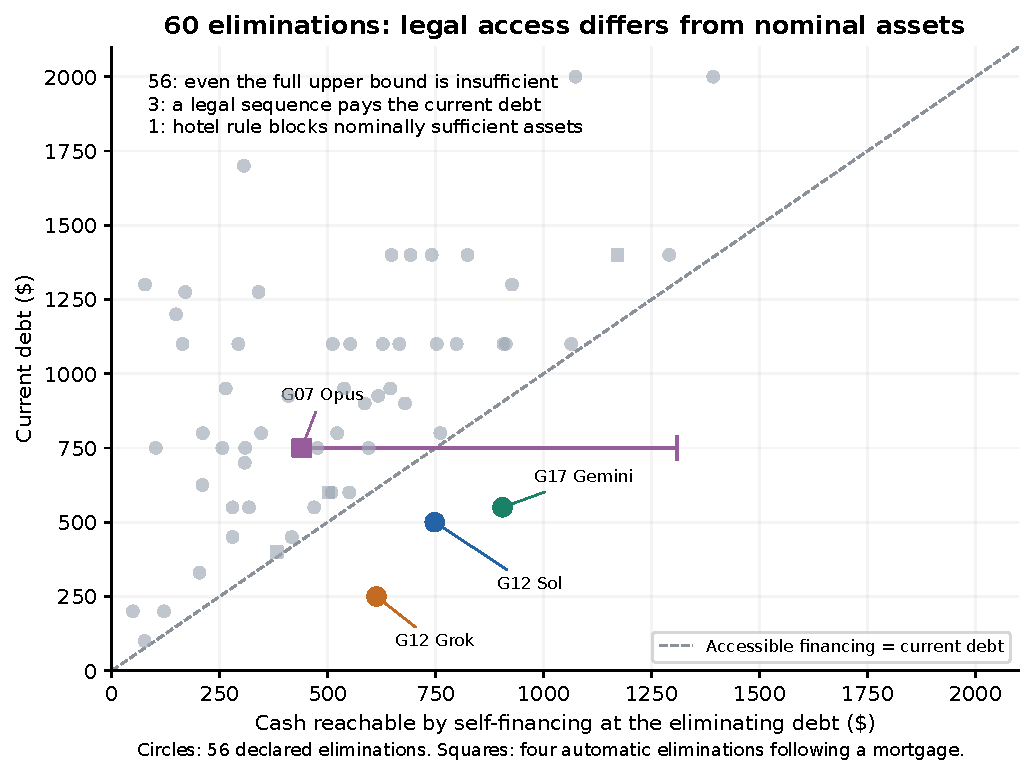
\includegraphics[width=\linewidth,height=0.57\textheight,keepaspectratio]{f06_elimination_financing.pdf}
\caption[Current-debt finance at all eliminations]{Each point is one applied elimination, including four automatic eliminations after mortgages. Horizontal position is cash accessible through the acting debtor's own legal liquidation sequence at that debt, without assuming help from another player. Vertical position is debt owed. In 56 cases even a generous full-access upper bound is insufficient. Three have engine-verified payment sequences; their mechanisms differ, including a contradictory received declaration in G12. In G7 the horizontal segment separates \$440 accessible from \$1,310 nominal under a \$750 debt because the hotel-sale rule binds. The greedy legal route reaches the full upper bound in 59 cases; maximality in the remaining case follows from exhausting both permitted mortgage orders and the empty sale menu. No claim is made about rational surrender, future survival, an alternative winner or the effect of earlier house retention. Source: Opus's all-elimination reconstruction with Astra/Sol exact-prefix checks and Fable's independent bounds.

F6 encoding note: circles are the 56 declared eliminations; squares are the four automatic eliminations after mortgages. All 60 observations are retained, including overlapping values. Highlight labels use leader lines without opaque boxes; the \$748/\$500 Sol point remains visible.}
\label{fig:f06_elimination_financing}
\end{figure}
% Native data cross-reference
\tablenote{Underlying data: Table~\ref{tab:t06_eliminations}.}
